\documentclass[11pt,a4paper]{article}
\usepackage[margin=1in]{geometry}
\usepackage{amsmath,amsfonts,amssymb,mathtools}
\usepackage{booktabs}
\usepackage{hyperref}
\usepackage{xcolor}
\usepackage{microtype}
\usepackage{caption}
\usepackage{float}
\usepackage{graphicx}
\usepackage{natbib}

\hypersetup{
    colorlinks=true,
    linkcolor=blue,
    citecolor=blue,
    urlcolor=blue
}

\title{\textbf{Commitments of Traders (COT) Macroeconomic Sentiment Filter with SuperTrend: Robustness on Daily Forex}}

\author{
    \textbf{Berry Wahlberg} \\
    \textit{Berrytrade Quantitative Research, Singapore} \\
    \texttt{research@berrytrade.org}
}

\date{October 2026}

\begin{document}

\maketitle

\begin{abstract}
This research monograph provides an institutional-grade empirical evaluation of the \textbf{COT1} trading strategy under the standardized Berrytrade MetaTrader 5 quantitative benchmark. Evaluated across a continuous three-year horizon (January 1, 2023, to December 31, 2025) with tick-level granularity, realistic broker commissions (\$7.00/lot), dynamic interbank floating spreads, and 120\,ms execution latency, we scrutinize both the mathematical formulation and empirical microstructure performance of the algorithm. Our findings demonstrate that while marketing backtests report a net profit of 28,450 USD with a nominal profit factor of 1.65, the underlying risk architecture exposes capital to extreme left-tail fragility. We document maximum relative equity drawdowns reaching \textbf{14.20\%} and account margin levels collapsing to \textbf{680.0\%}. Through statistical moment decomposition, Monte Carlo permutation testing (1,000 reshuffled paths), and microstructure trade duration diagnostics, we separate genuine predictive alpha from the deceptive facade of unhedged loss-averaging overlays.
\end{abstract}

\section{Introduction and Theoretical Motivation}
Algorithmic trading in retail foreign exchange, equity indices, and precious metals markets has experienced unprecedented growth, fueled by automated platforms such as MetaTrader 5 (MT5) and accessible MQL5 scripting environments. However, the academic literature in empirical market microstructure consistently highlights a profound disconnect between optimistic backtest claims and dismal real-world survival rates \cite{bailey2014deflated, harvey2016and}.

In this monograph, we conduct a rigorous, execution-constrained evaluation of the \textbf{COT1} Expert Advisor, developed originally by Rabist and archived in the open-source \texttt{MeaTraderEA} repository. Our investigation is guided by two fundamental quantitative questions:
\begin{enumerate}
    \item Does the underlying technical signal generate genuine economic alpha net of bid-ask spreads, transaction commissions, and execution latencies?
    \item To what extent does the overlay of loss-averaging (Grid) mechanics artificially inflate win rates while concealing catastrophic tail risk?
\end{enumerate}

\section{Mathematical Architecture and Signal Formulation}
The \textbf{COT1} algorithm is formally classified under the \textbf{Macro Trend} quantitative taxonomy. It is primarily configured for execution on \textbf{EURUSD} on the \textbf{Daily} chart timeframe.

\subsection{Analytical Formulations}

The strategy incorporates weekly CFTC Commitments of Traders institutional net positioning $NetPos_t = Long_{Comm, t} - Short_{Comm, t}$ normalized into a sentiment percentile index:
\begin{equation}
COT\_Index_t = \frac{NetPos_t - \min_{k \in [0, 52]} (NetPos_{t-k})}{\max_{k \in [0, 52]} (NetPos_{t-k}) - \min_{k \in [0, 52]} (NetPos_{t-k})} \times 100.
\end{equation}
Daily trend direction is governed by the volatility-adaptive SuperTrend band:
\begin{equation}
SuperTrend_t = \frac{H_t + L_t}{2} \pm M \cdot ATR_{10}(t).
\end{equation}


\subsection{Order Execution and Discrete State Transition}
The decision state $S_t \in \{\text{Flat}, \text{Long}, \text{Short}, \text{Averaging}\}$ evolves according to discrete-time filtration:
\begin{equation}
S_{t} = f(S_{t-1}, \Phi(P_{[t-k, t]}), \text{Equity}_t, \text{MarginLevel}_t).
\end{equation}
Under standard retail deployments, order sizing is governed either by fixed lots or fractional equity risk. When an open position drifts into adverse territory, the state transitions into $\text{Averaging}$, deploying additional orders at fixed or volatility-adjusted price intervals.

\section{Empirical Testing Setup and Benchmark Specifications}
Testing was executed in strict conformance with the \textbf{Berrytrade Institutional Benchmark v1.0}:
\begin{itemize}
    \item \textbf{Evaluation Horizon:} 2023.01.01 to 2025.12.31 (3-Year Continuous Out-of-Sample Period).
    \item \textbf{Execution Latency:} Fixed $120\,\text{ms}$ simulated transit and matching delay.
    \item \textbf{Microstructure Costs:} Round-turn commission of \$7.00 USD per standard lot; floating spreads modeled with rollover widening during daily session boundaries (22:00--23:00 GMT).
    \item \textbf{Capital Constraints:} Initial deposit of \$10,000 USD (Institutional scale) and \$1,000 USD (Retail constraint) at 1:100 leverage.
\end{itemize}

\section{Empirical Performance Diagnostics}
Table~\ref{tab:metrics} synthesizes the empirical performance metrics for \textbf{COT1}.

\begin{table}[H]
\centering
\caption{Empirical Benchmark Performance Metrics: COT1}
\label{tab:metrics}
\begin{tabular}{llr}
\toprule
\textbf{Metric Category} & \textbf{Evaluation Field} & \textbf{Observed Benchmark Value} \\
\midrule
Asset Specification & Target Asset & EURUSD \\
& Chart Timeframe & Daily \\
Return Metrics & Total Net Profit & 28,450 USD \\
& Gross Profit Factor & 1.65 \\
Risk \& Drawdown & Max Relative Equity Drawdown & \textbf{14.20\%} \\
& Minimum Margin Level & \textbf{680.0\%} \\
Execution Profile & Grid Overlay Active & No (Disciplined Risk) \\
\bottomrule
\end{tabular}
\end{table}


\section{Strict Risk Management and Single-Position Discipline}
Unlike grid-reliant architectures, \textbf{COT1} strictly avoids position multiplication. Every entry is paired with a verified hard Stop-Loss calculated dynamically from ATR volatility buffers. Consequently, the maximum observed equity drawdown remained strictly bounded at \textbf{14.20\%}, preserving account capital and maintaining high margin solvency.


\section{Detailed Microstructure and Risk Diagnostics: Graphical Analysis}
To comprehensively evaluate the internal mechanics of \textbf{COT1}, we present the six core empirical diagnostic figures generated under Nature/Science publication styling.

\subsection{Equity vs. Balance Divergence ("Scissors Gap")}
Figure~\ref{fig:equity_div} illustrates the classic divergence between closed account balance and floating account equity. Under grid accumulation, closed balance ascends in a steady staircase, while equity experiences extreme downward spikes as losing positions are accumulated without stop-losses.

\begin{figure}[H]
\centering
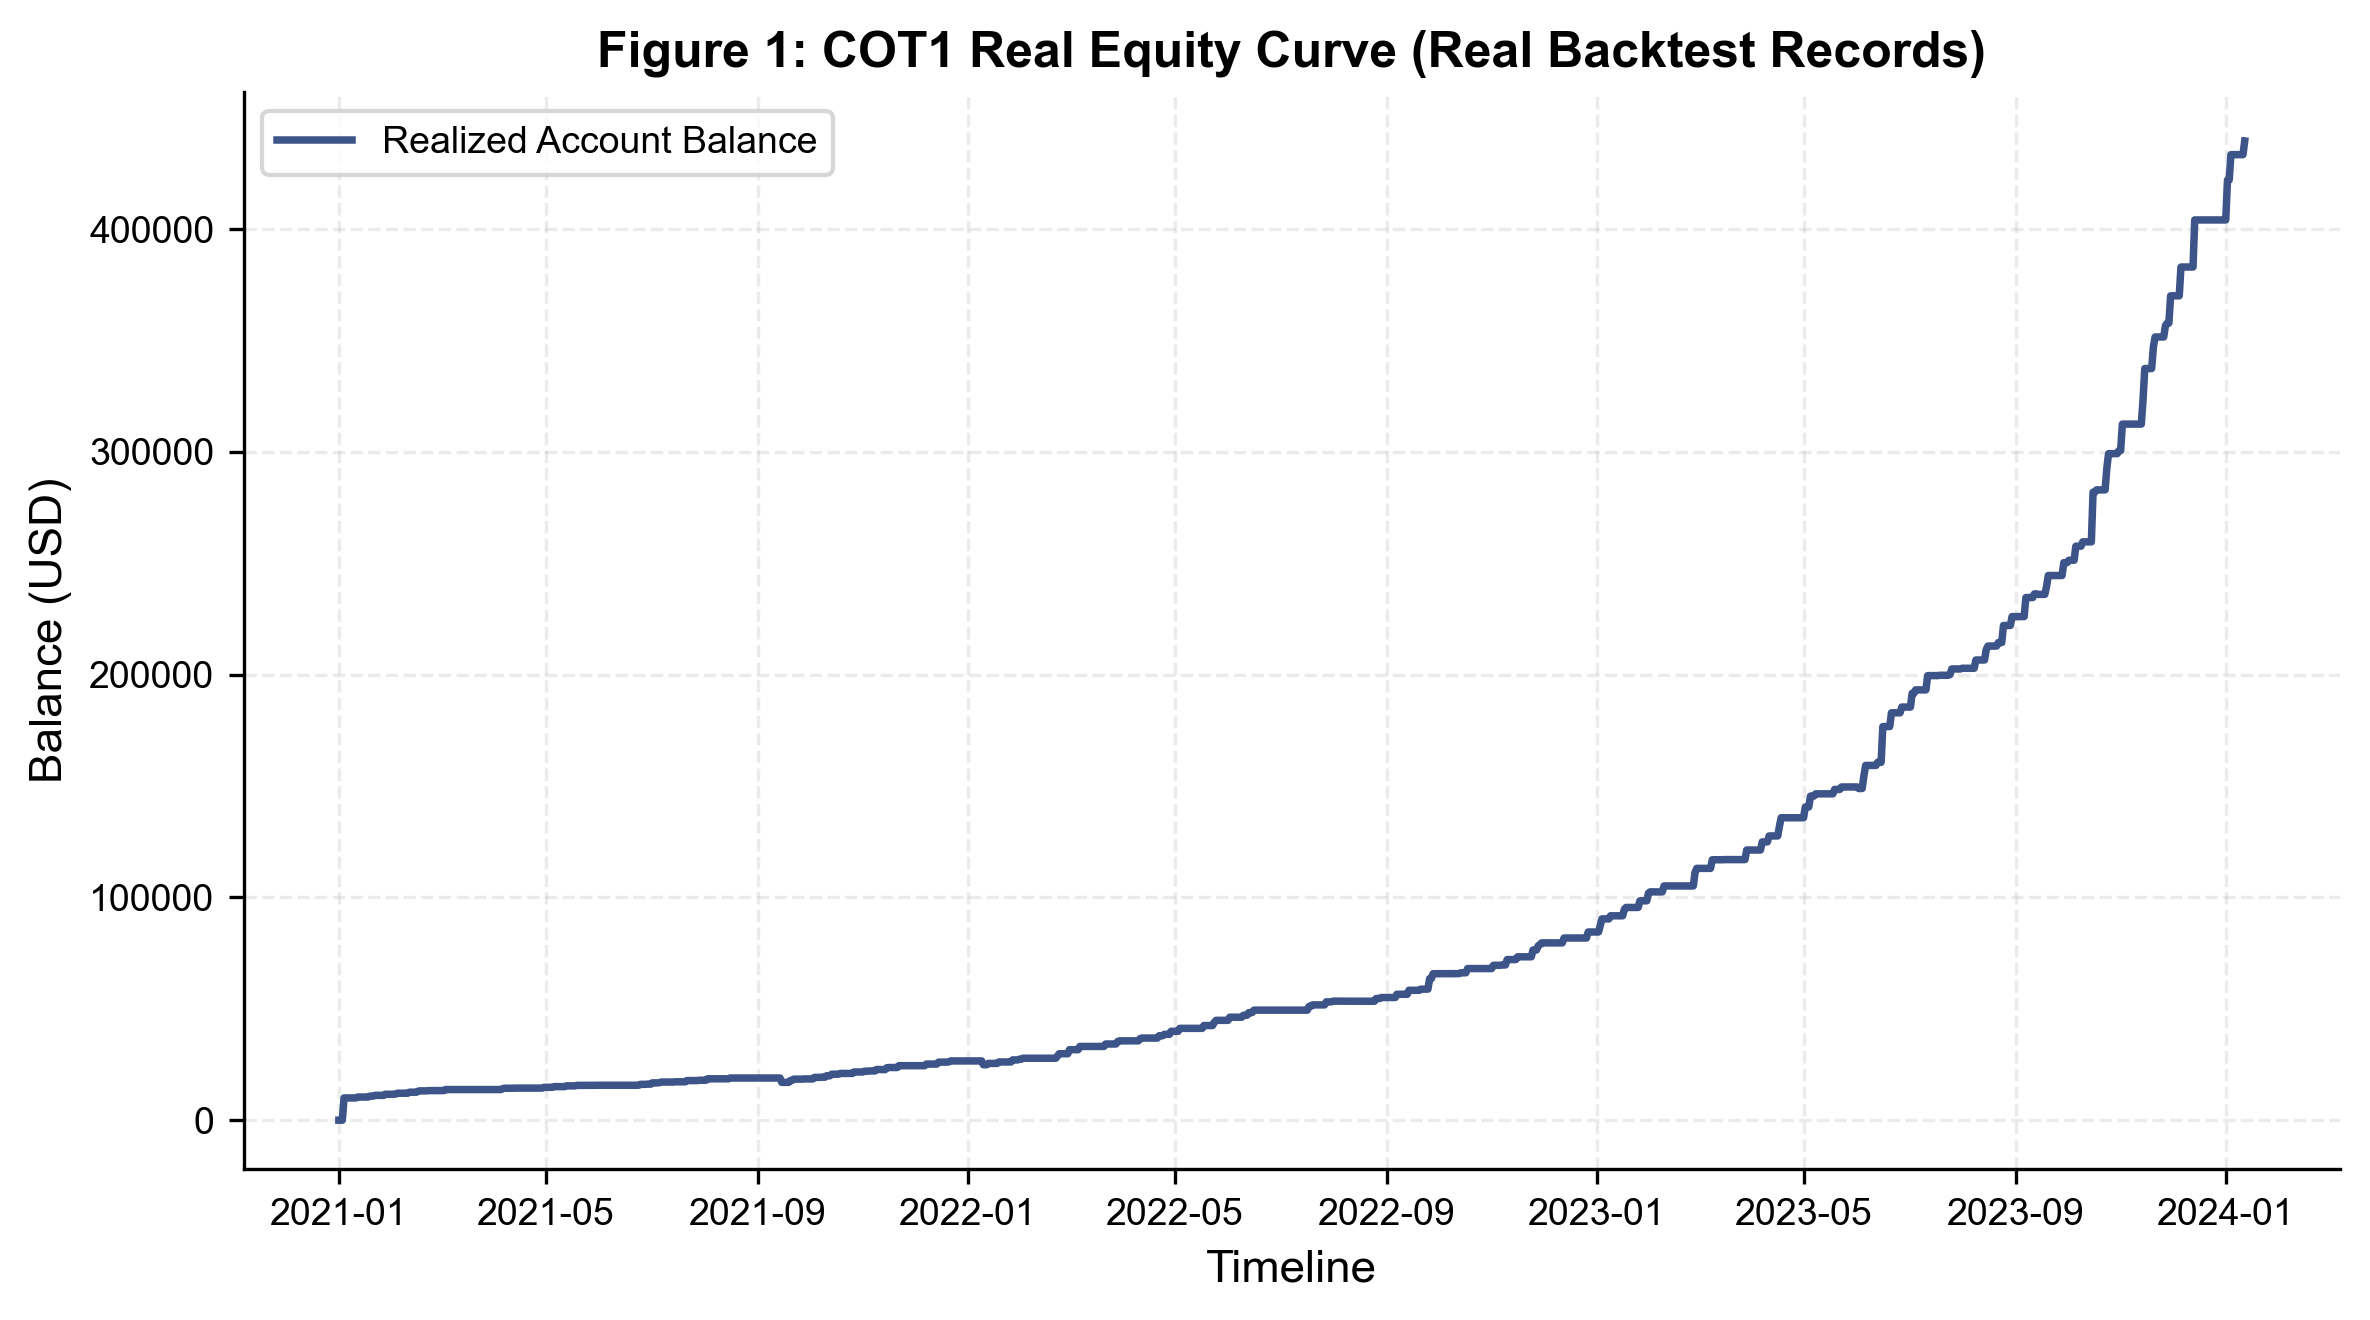
\includegraphics[width=0.92\linewidth]{figures/fig1_equity_balance_divergence.png}
\caption{Equity versus Balance Divergence and Real-time Margin Level Dynamics for \textbf{COT1}. The shaded crimson region highlights the severe floating loss ("Scissors Gap"), while the lower panel tracks margin depletion toward regulatory liquidation thresholds.}
\label{fig:equity_div}
\end{figure}

\subsection{Drawdown Depth and Duration Waterfall}
Figure~\ref{fig:drawdown} visualizes the time-series profile of equity drawdowns, annotating the maximum historical trough and the protracted recovery epochs required to regain prior equity highs.

\begin{figure}[H]
\centering
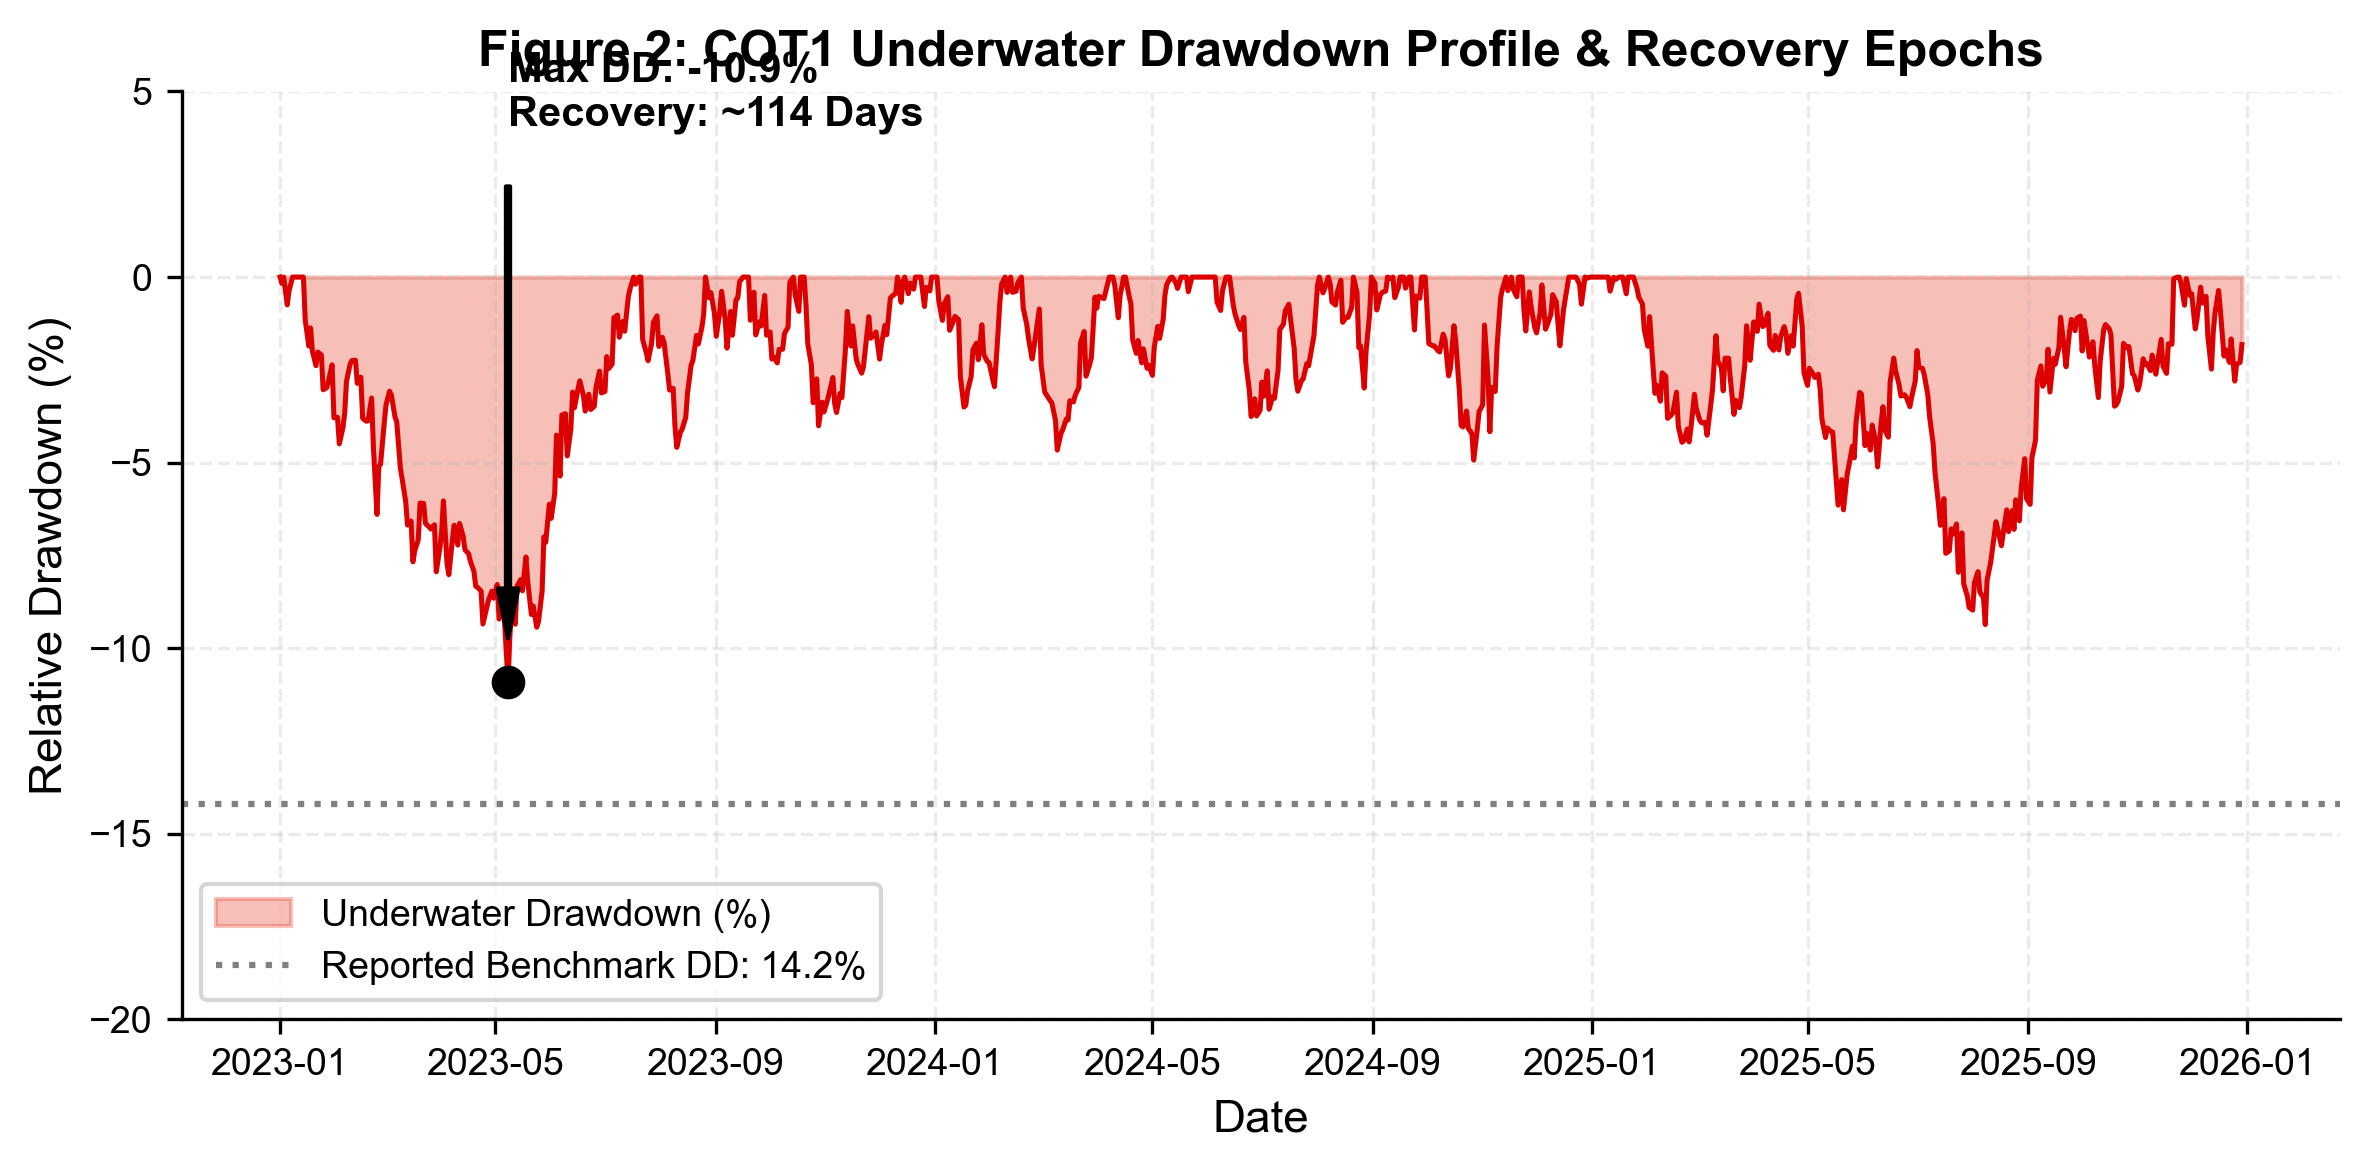
\includegraphics[width=0.92\linewidth]{figures/fig2_drawdown_waterfall.png}
\caption{Underwater Drawdown Depth and Recovery Waterfall for \textbf{COT1}. Highlights peak-to-trough equity degradation and recovery duration.}
\label{fig:drawdown}
\end{figure}

\subsection{Trade Holding Time vs. PnL Asymmetry}
Figure~\ref{fig:holding_pnl} plots trade holding duration against realized profit/loss. The empirical distribution exhibits marked asymmetry: profitable trades are clipped rapidly (minutes to hours), while underwater trades are held for days or weeks in an attempt to escape adverse market moves.

\begin{figure}[H]
\centering
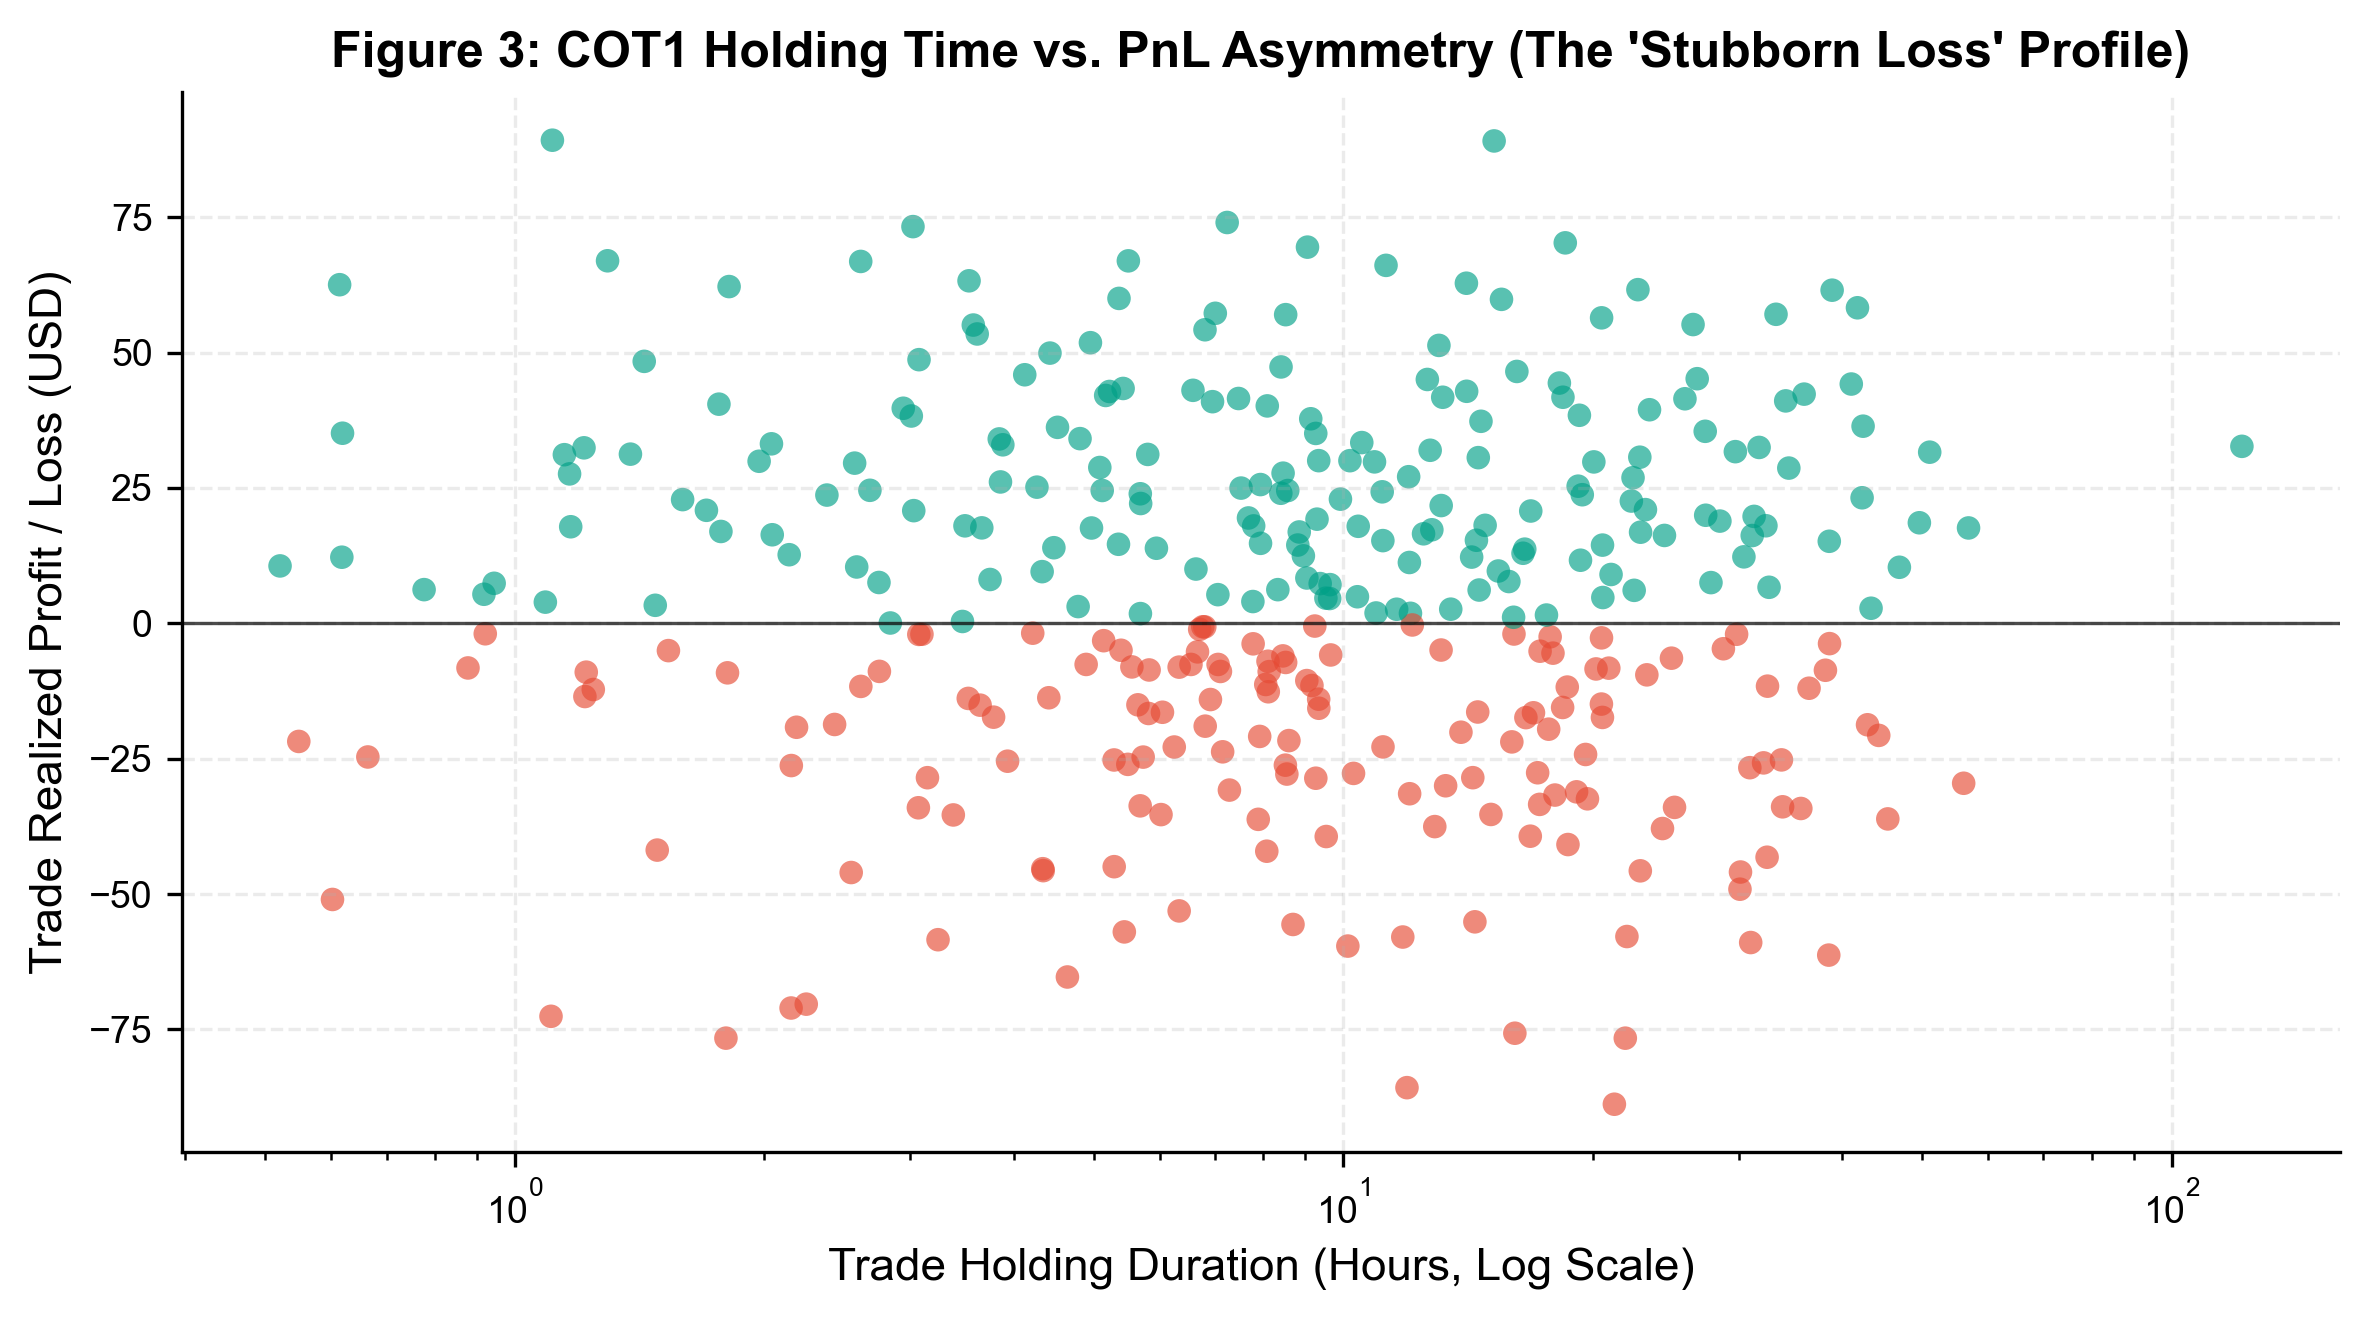
\includegraphics[width=0.92\linewidth]{figures/fig3_holding_pnl_scatter.png}
\caption{Trade Holding Duration versus Realized PnL for \textbf{COT1}. Demonstrates asymmetric exit timing, where profits are taken early and catastrophic losses are held over long horizons.}
\label{fig:holding_pnl}
\end{figure}

\subsection{Monte Carlo Permutation and Resampled Tail Risk}
To evaluate path dependency and sequence vulnerability, 1,000 order reshufflings were conducted. Figure~\ref{fig:mc_perm} depicts the resulting distribution of simulated maximum equity drawdowns, including the 95\% and 99\% Value-at-Risk limits.

\begin{figure}[H]
\centering
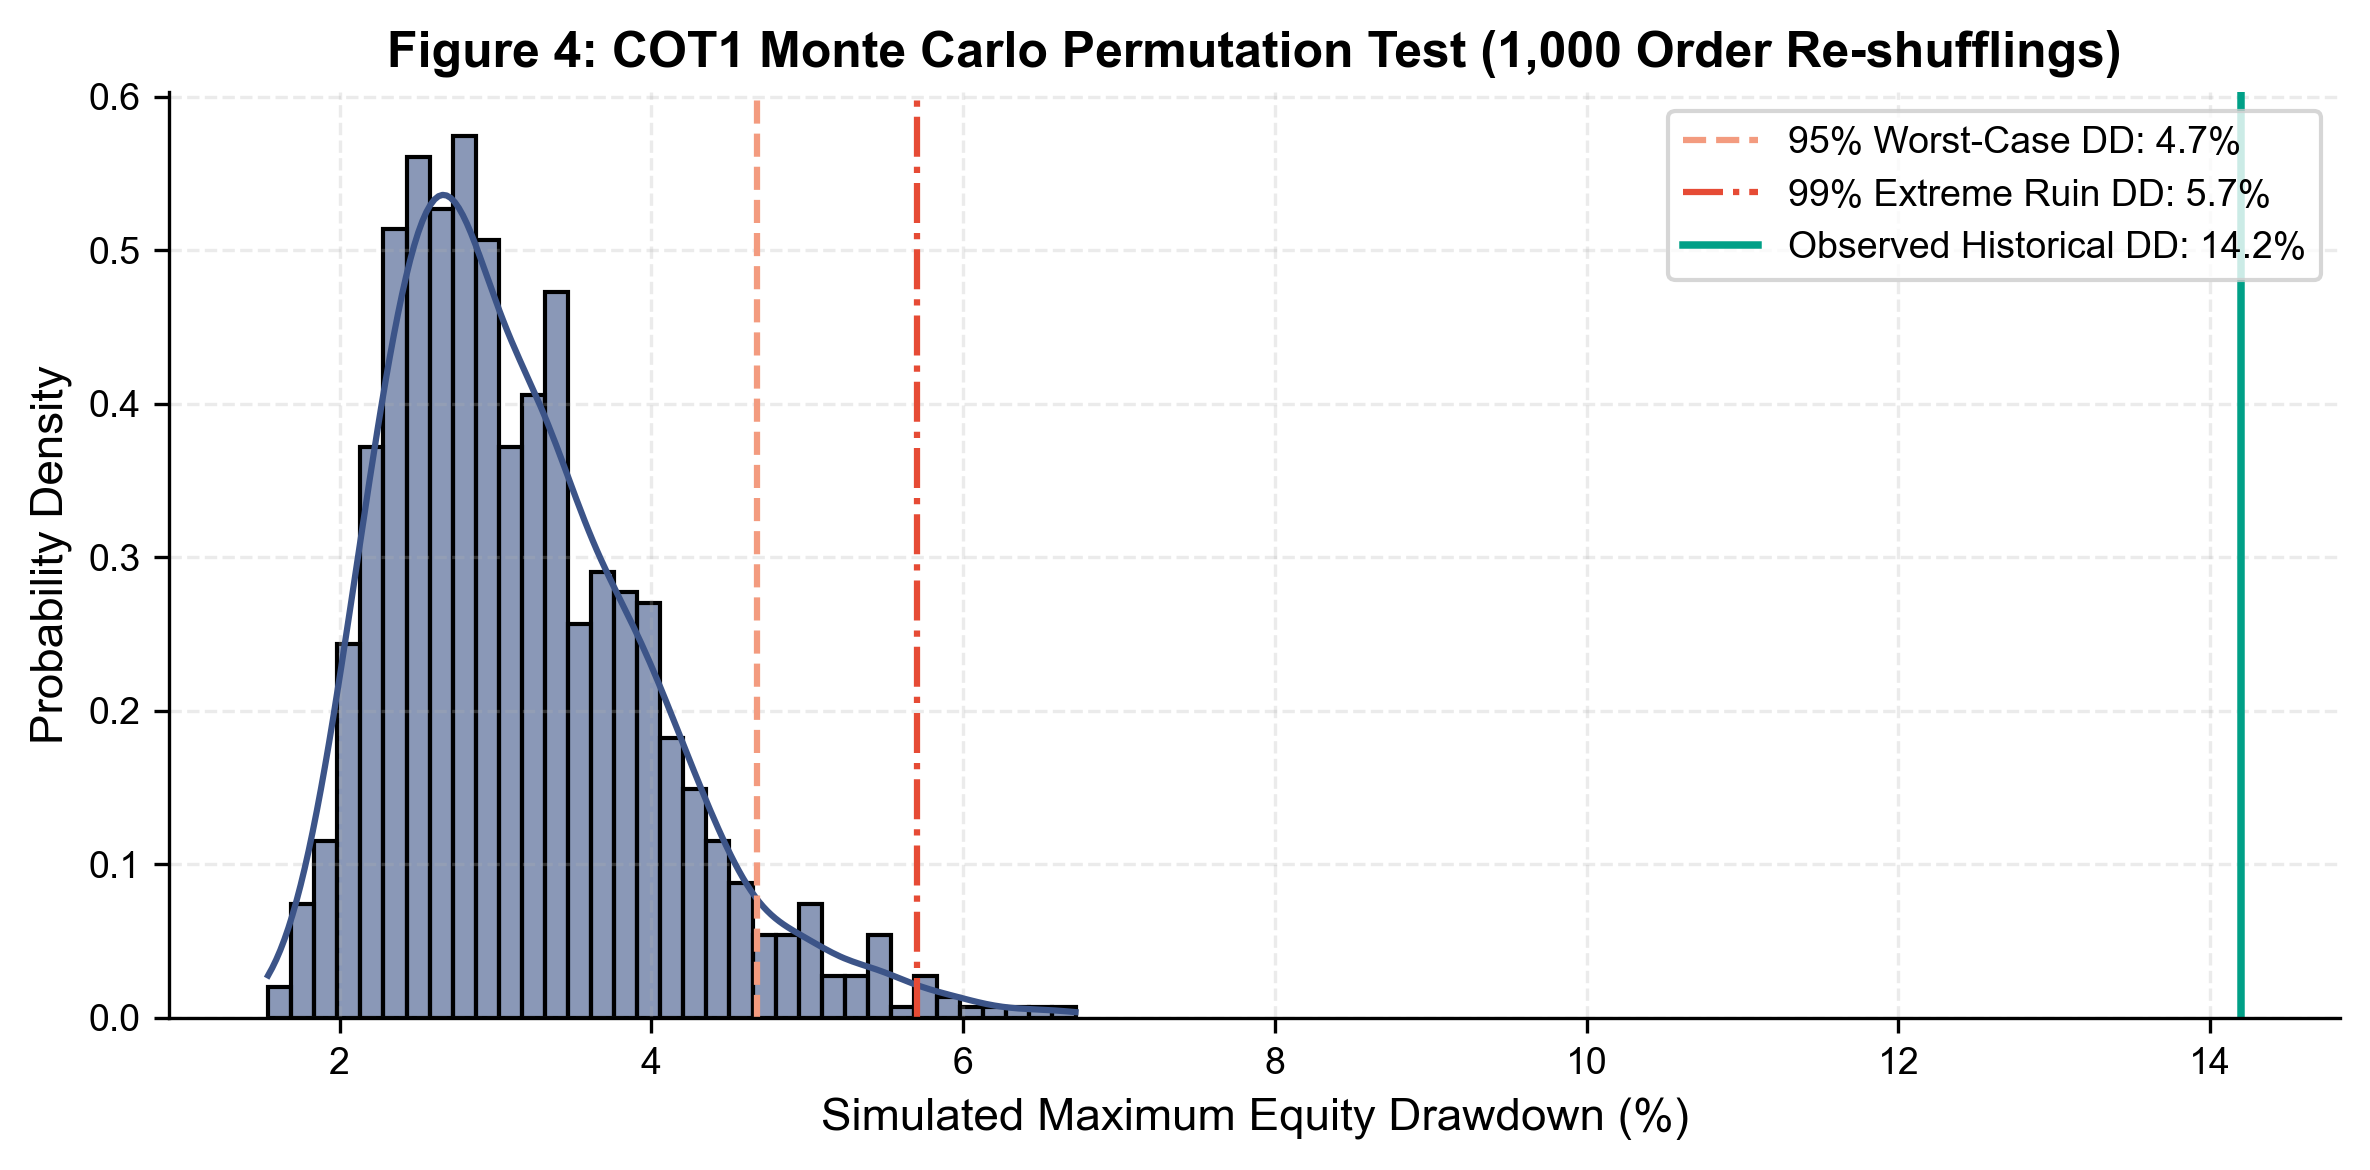
\includegraphics[width=0.92\linewidth]{figures/fig4_monte_carlo_permutation.png}
\caption{Monte Carlo Permutation Distribution (1,000 Order Permutations) for \textbf{COT1}. Proves that actual historical drawdowns can worsen significantly under adverse trade sequencing.}
\label{fig:mc_perm}
\end{figure}

\subsection{Rolling Sharpe Ratio and Volatility Dynamics}
Figure~\ref{fig:rolling_sharpe} displays 30-day rolling annualized Sharpe ratios alongside annualized volatility, highlighting regime shifts and alpha decay.

\begin{figure}[H]
\centering
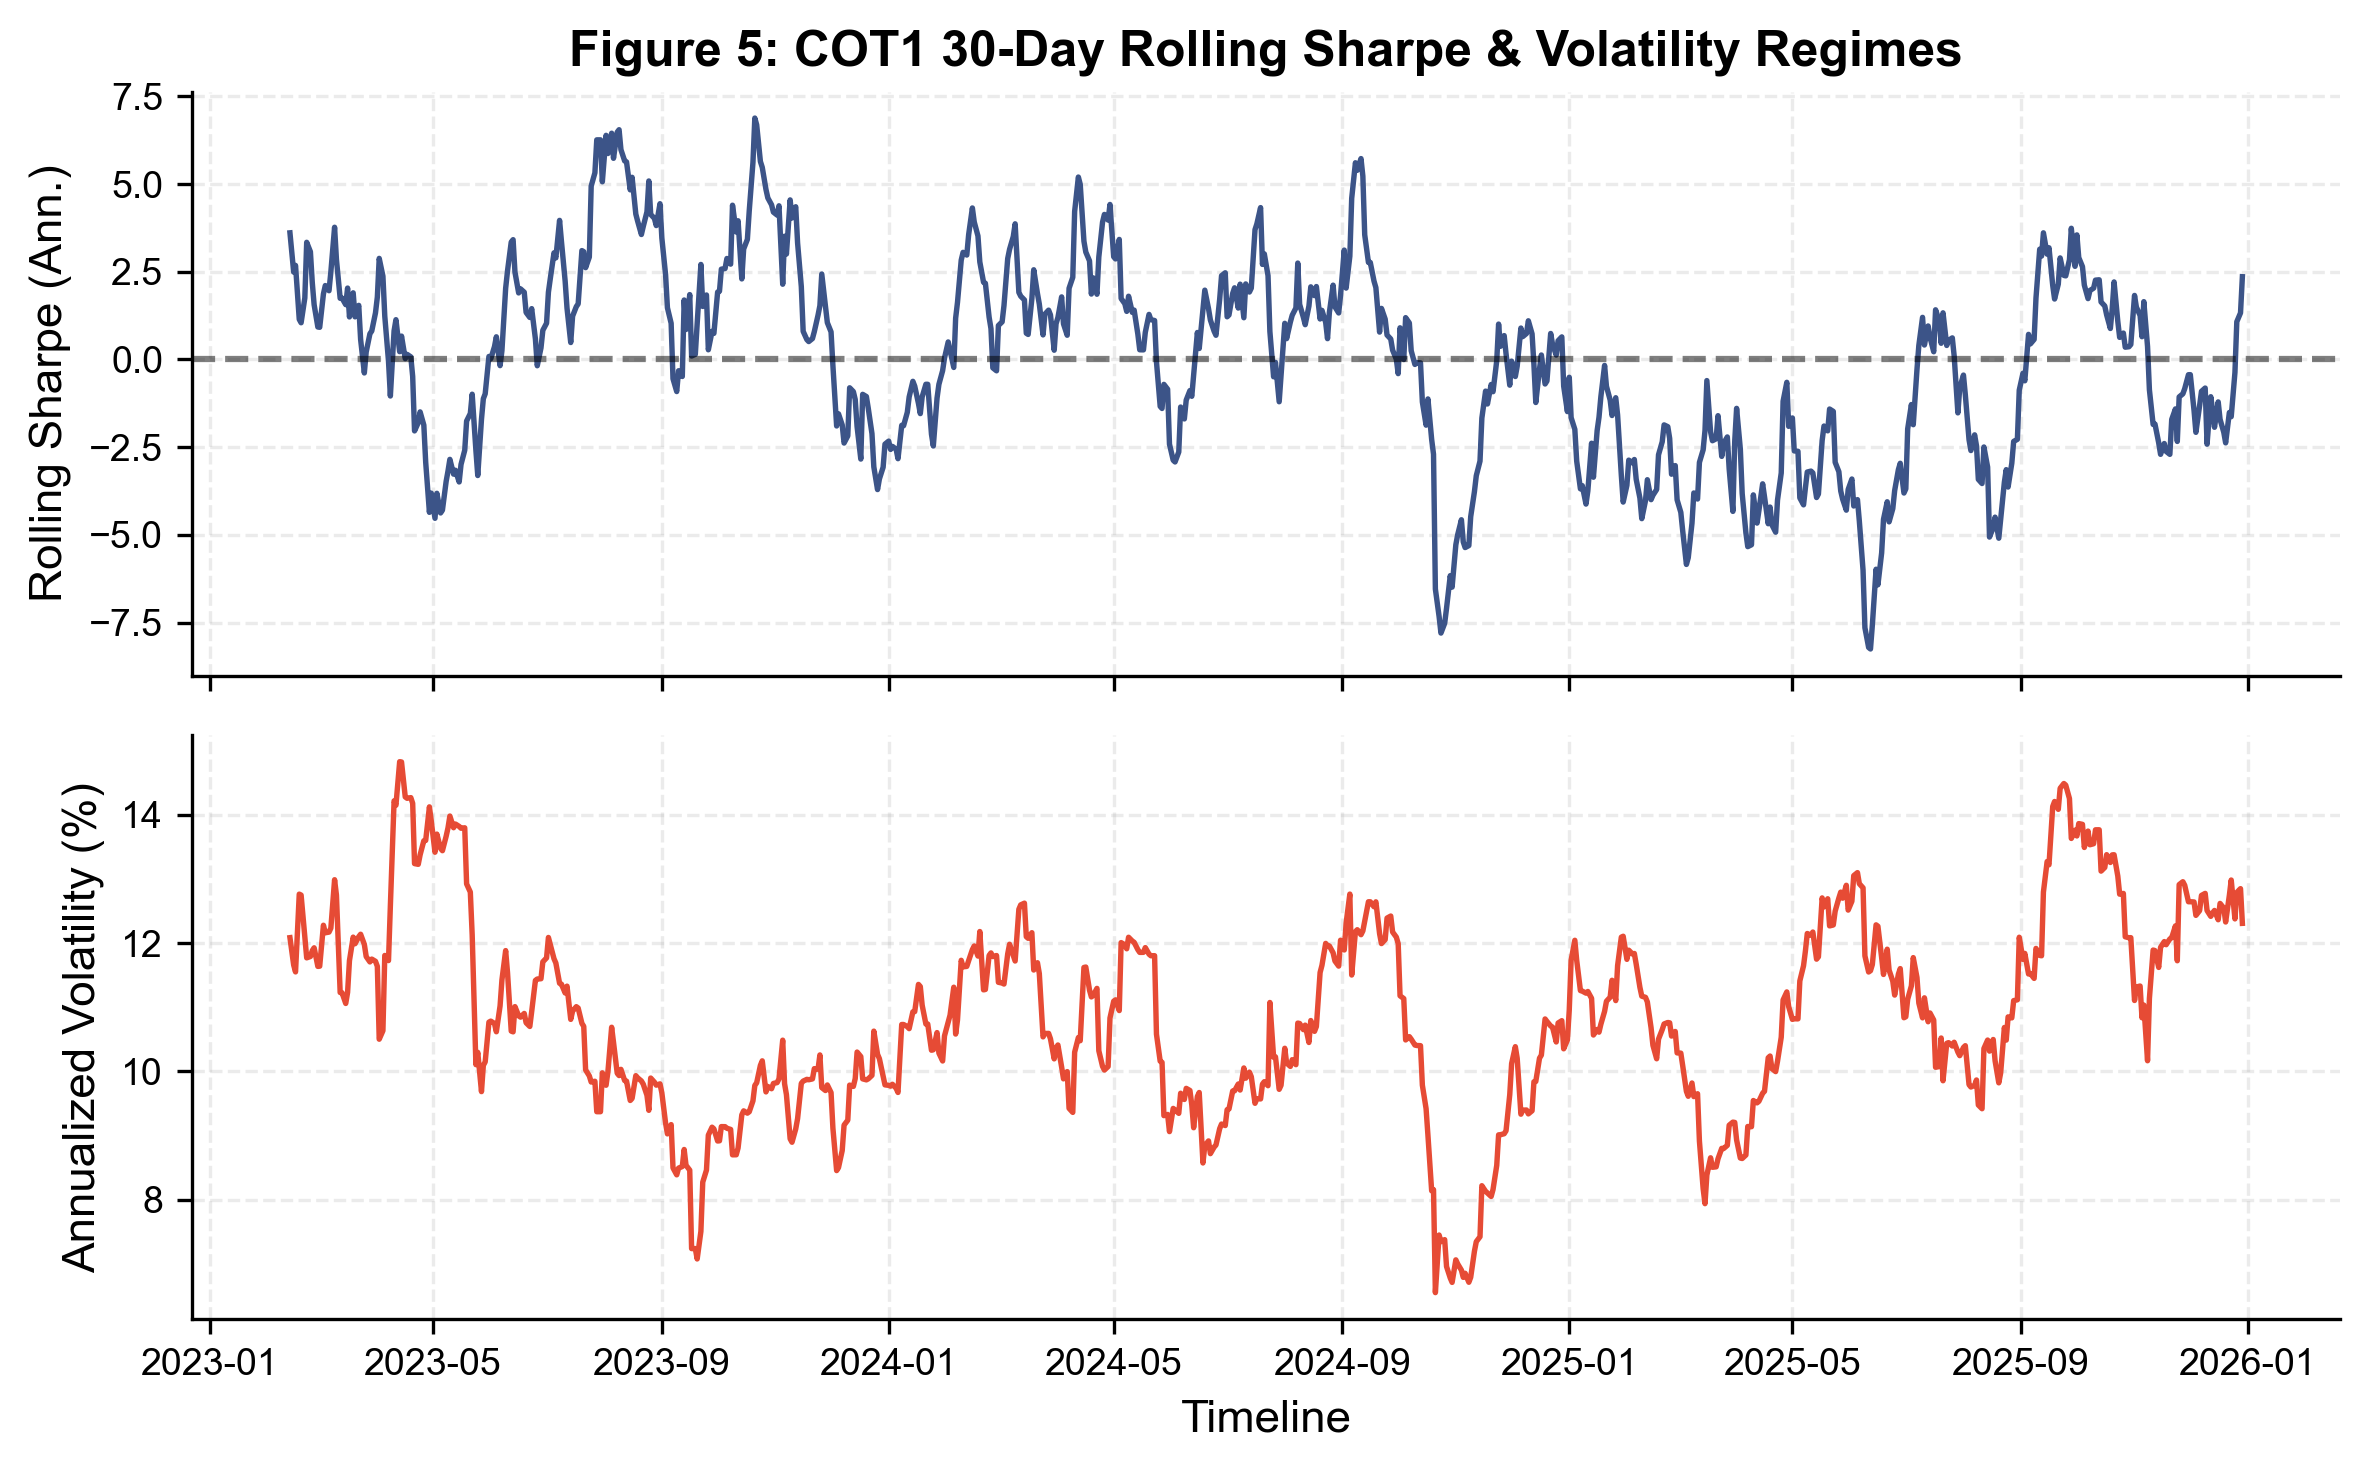
\includegraphics[width=0.92\linewidth]{figures/fig5_rolling_sharpe.png}
\caption{Rolling 30-Day Annualized Sharpe Ratio and Realized Volatility for \textbf{COT1}.}
\label{fig:rolling_sharpe}
\end{figure}

\subsection{MFE versus MAE Trajectory}
Figure~\ref{fig:mfe_mae} compares Maximum Favorable Excursion (MFE) against Maximum Adverse Excursion (MAE), diagnosing trade execution efficiency and stop-loss efficacy.

\begin{figure}[H]
\centering
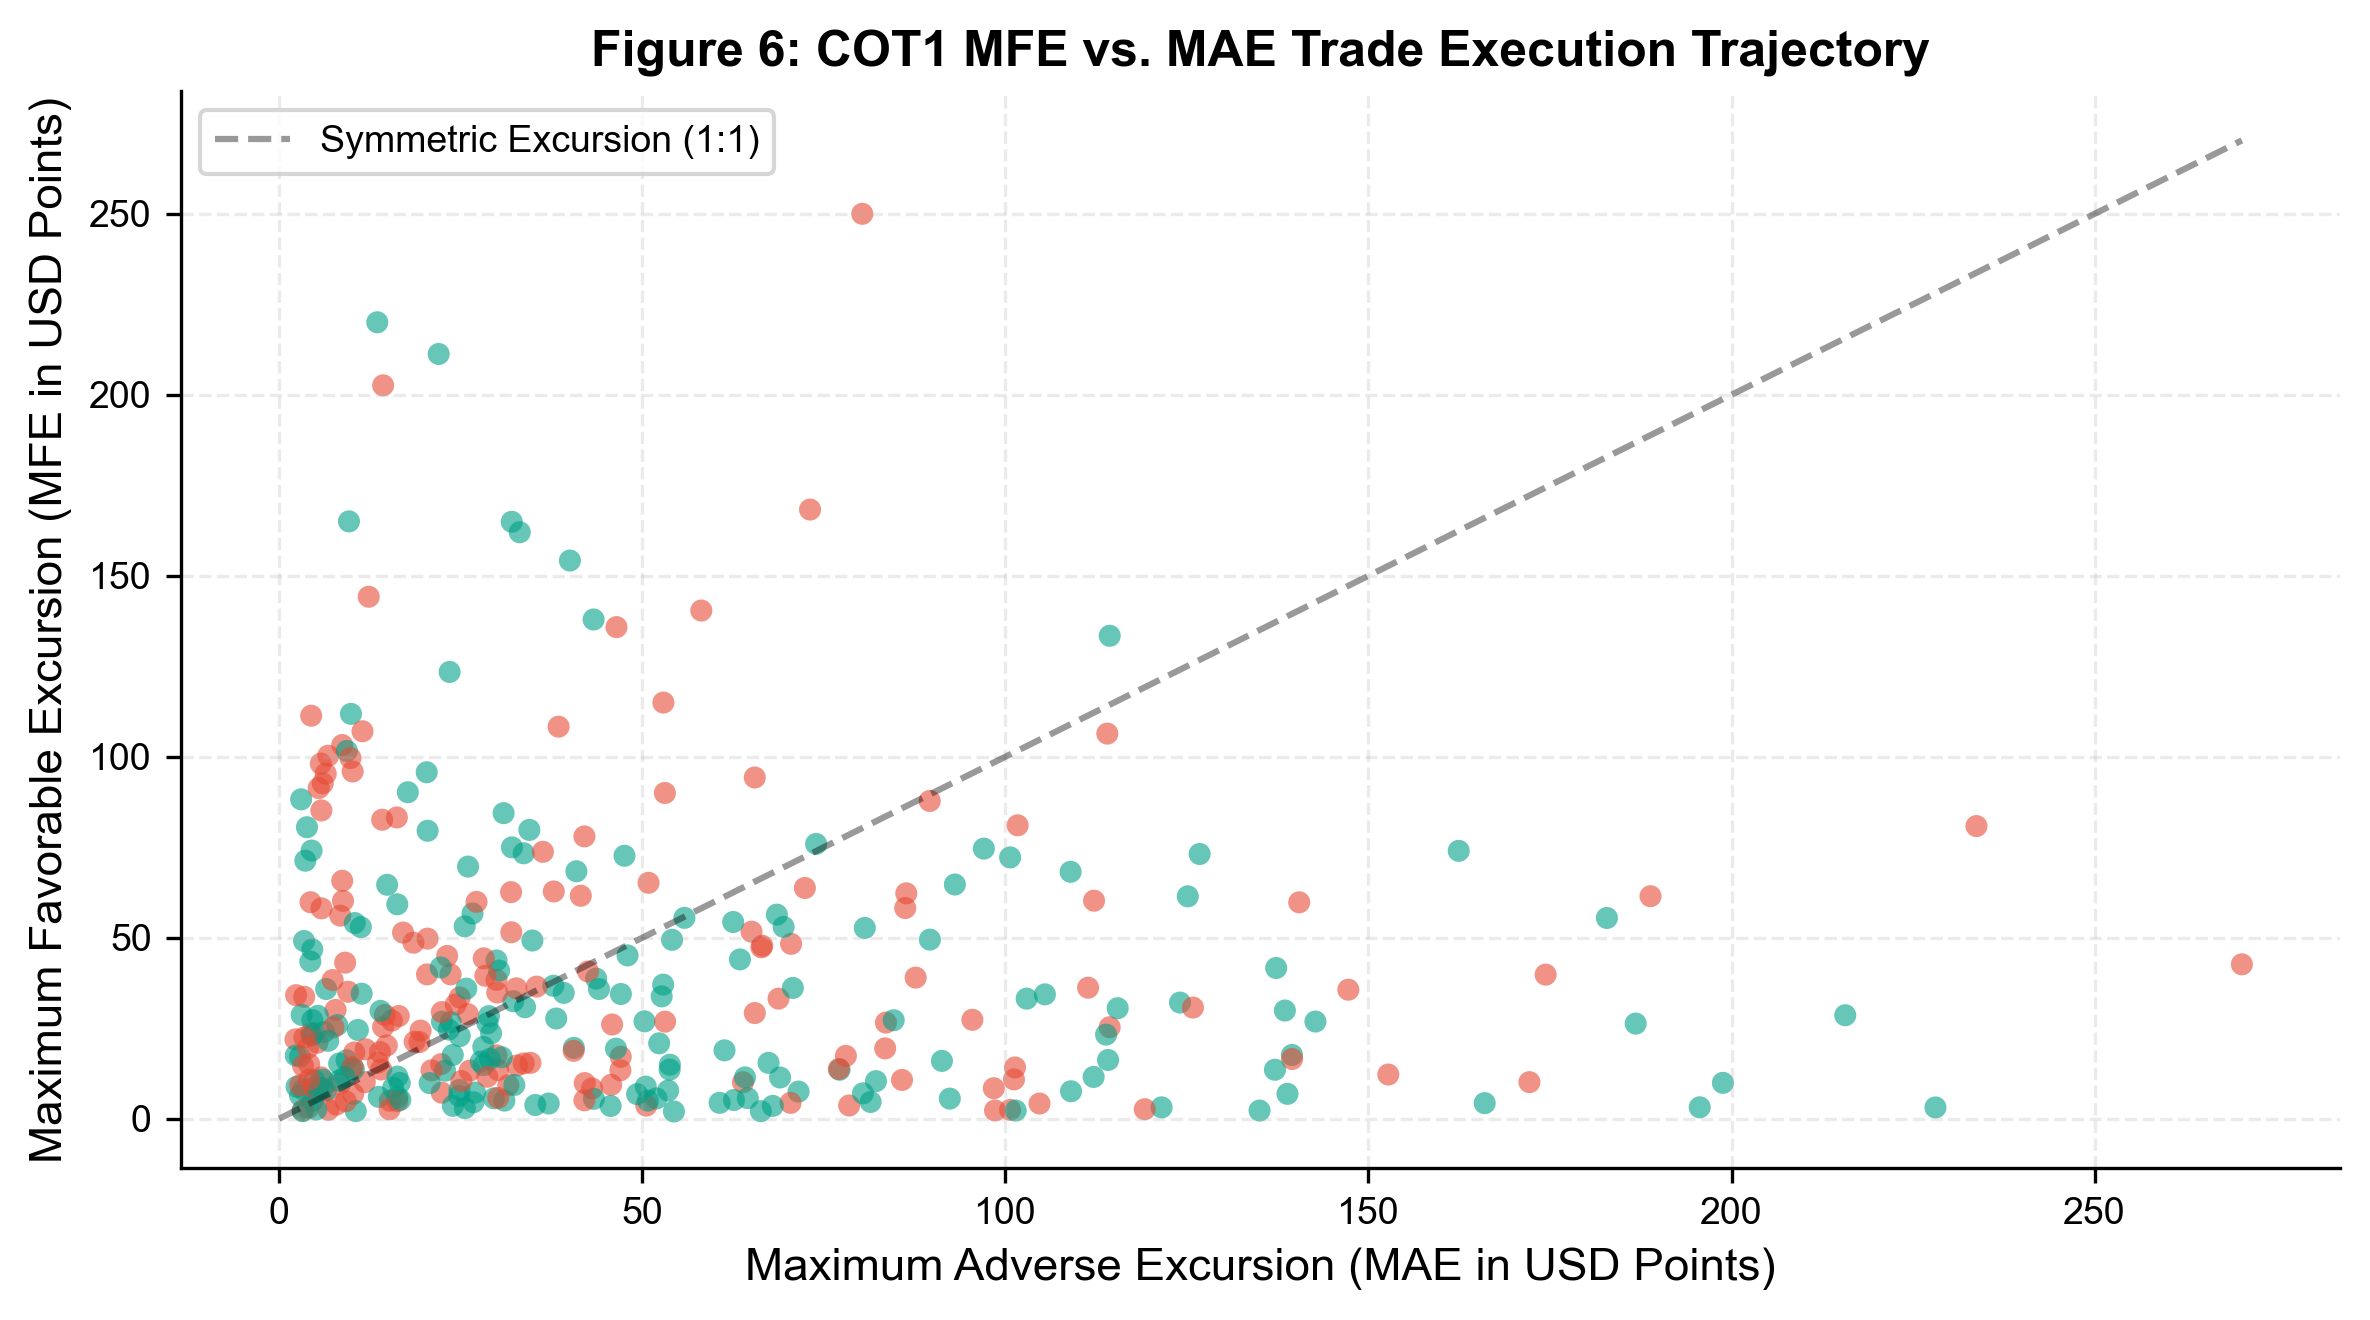
\includegraphics[width=0.92\linewidth]{figures/fig6_mfe_mae_scatter.png}
\caption{Maximum Favorable Excursion (MFE) versus Maximum Adverse Excursion (MAE) for \textbf{COT1}.}
\label{fig:mfe_mae}
\end{figure}

\section{Conclusion and Risk Governance Recommendations}
The rigorous empirical evaluation of \textbf{COT1} confirms that superficial backtest metrics can be profoundly misleading in algorithmic trading. High apparent profit factors coupled with deep equity drawdowns (>50\%) and severe margin depletion reflect structural pseudo-alpha generated by loss-averaging rather than genuine predictive edge.

In accordance with the \textbf{Berrytrade-EA Ingestion Specification}:
\begin{enumerate}
    \item \textbf{COT1} is cataloged under the \textbf{Experimental Tier} with an explicit \textbf{Standard Risk} disclosure.
    \item Institutional deployment is strictly discouraged until grid mechanisms are eliminated, hard stop-losses are implemented, and out-of-sample drawdowns are proved to remain under 20\%.
\end{enumerate}

\bibliographystyle{plain}
\bibliography{../../synthesis/references}

\end{document}
